\section{Sesión 5}

\begin{prop}
	Sea $f\in R[a,b]$. Entonces, $|f| \in R[a,b]$. Además, se tiene: 
	$$\left|\int_a^b f \right|\leq \int_a^b |f|.$$
\end{prop}

\begin{nota}
	\begin{enumerate}
		\item Si $f(x)\leq g(x),\forall x\in [a,b]$, se tiene que: $$\overline{\int_a^b }f\leq \overline{\int_a^b} g; \underline{\int_a^b }f\leq \underline{\int_a^b}g.$$
		\item $$\left|\overline{\int_a^b}f\right|\leq \overline{\int_a^b}|f|;\left|\underline{\int_a^b}f\right|\leq \underline{\int_a^b}|f| $$
	\end{enumerate}
\end{nota}

\begin{prop}
	Sea $f\in R[a,b]\implies f^2\in R[a,b]$. 
\end{prop}

\begin{teorema}
	Si $f, g\in R[a,b]\implies f\cdot g \in R[a,b]$. 
\end{teorema}

\begin{prop}
	Sean $f:[a,b]\to \mathbb{R}$ acotada y $m,M\in R\ni m\leq f(x)\leq M, \forall x\in [a,b]$. Entonces: 
	\begin{enumerate}
		\item $m(b-a)\leq \underline{\int_a^b}f$.
		\item $\overline{\int_a^b}f\leq M(b-a)$.
	\end{enumerate}
\end{prop}

\begin{teorema}(***)
	Sea $I$ un intervalo y $f:I\to \mathbb{R}$ una función continua en $I$. Sea $a\in I$ y considere las funciones: 
	
	$$\overline{F(x)}=\overline{\int_a^x}f \quad \text{y} \quad \underline{F(x)}=\underline{\int_a^x}f,\forall x\in I.$$
	Entonces: 
	\begin{enumerate}
		\item $\overline{F}$ y $\underline{F}$ son continuas en $I$. 
		\item Si $f$ es continua en $c\in I\implies \overline{F}$ y $\underline{F}$ son derivables en $c$ y además: 
		$$\overline{F}'(c)=\underline{F}'(c)=f(x).$$
	\end{enumerate}
\end{teorema}

\begin{teorema}(Primer teorema fundamental del cálculo)
	Sea $f\in R[a,b]$. Sea $F:[a,b]\to\mathbb{R}\ni$ 
	$$F(x):= \int_a^x f, \quad x[a,b]$$
	Si $f$ es continua en $c\in [a,b]\implies I$ es derivable en $c$ y $F'(c)=f(c)$. 
\end{teorema}

\begin{teorema}(Segundo teorema fundamental del cálculo- Fórmula Newton-Leibniz)
	Sea $f\in R[a,b]$ y sea $G$ una función derivable en $(a,b)\ni G'=f$. Entonces, 
	
	$$\int_a^b f=G(b)-G(a).$$
\end{teorema}
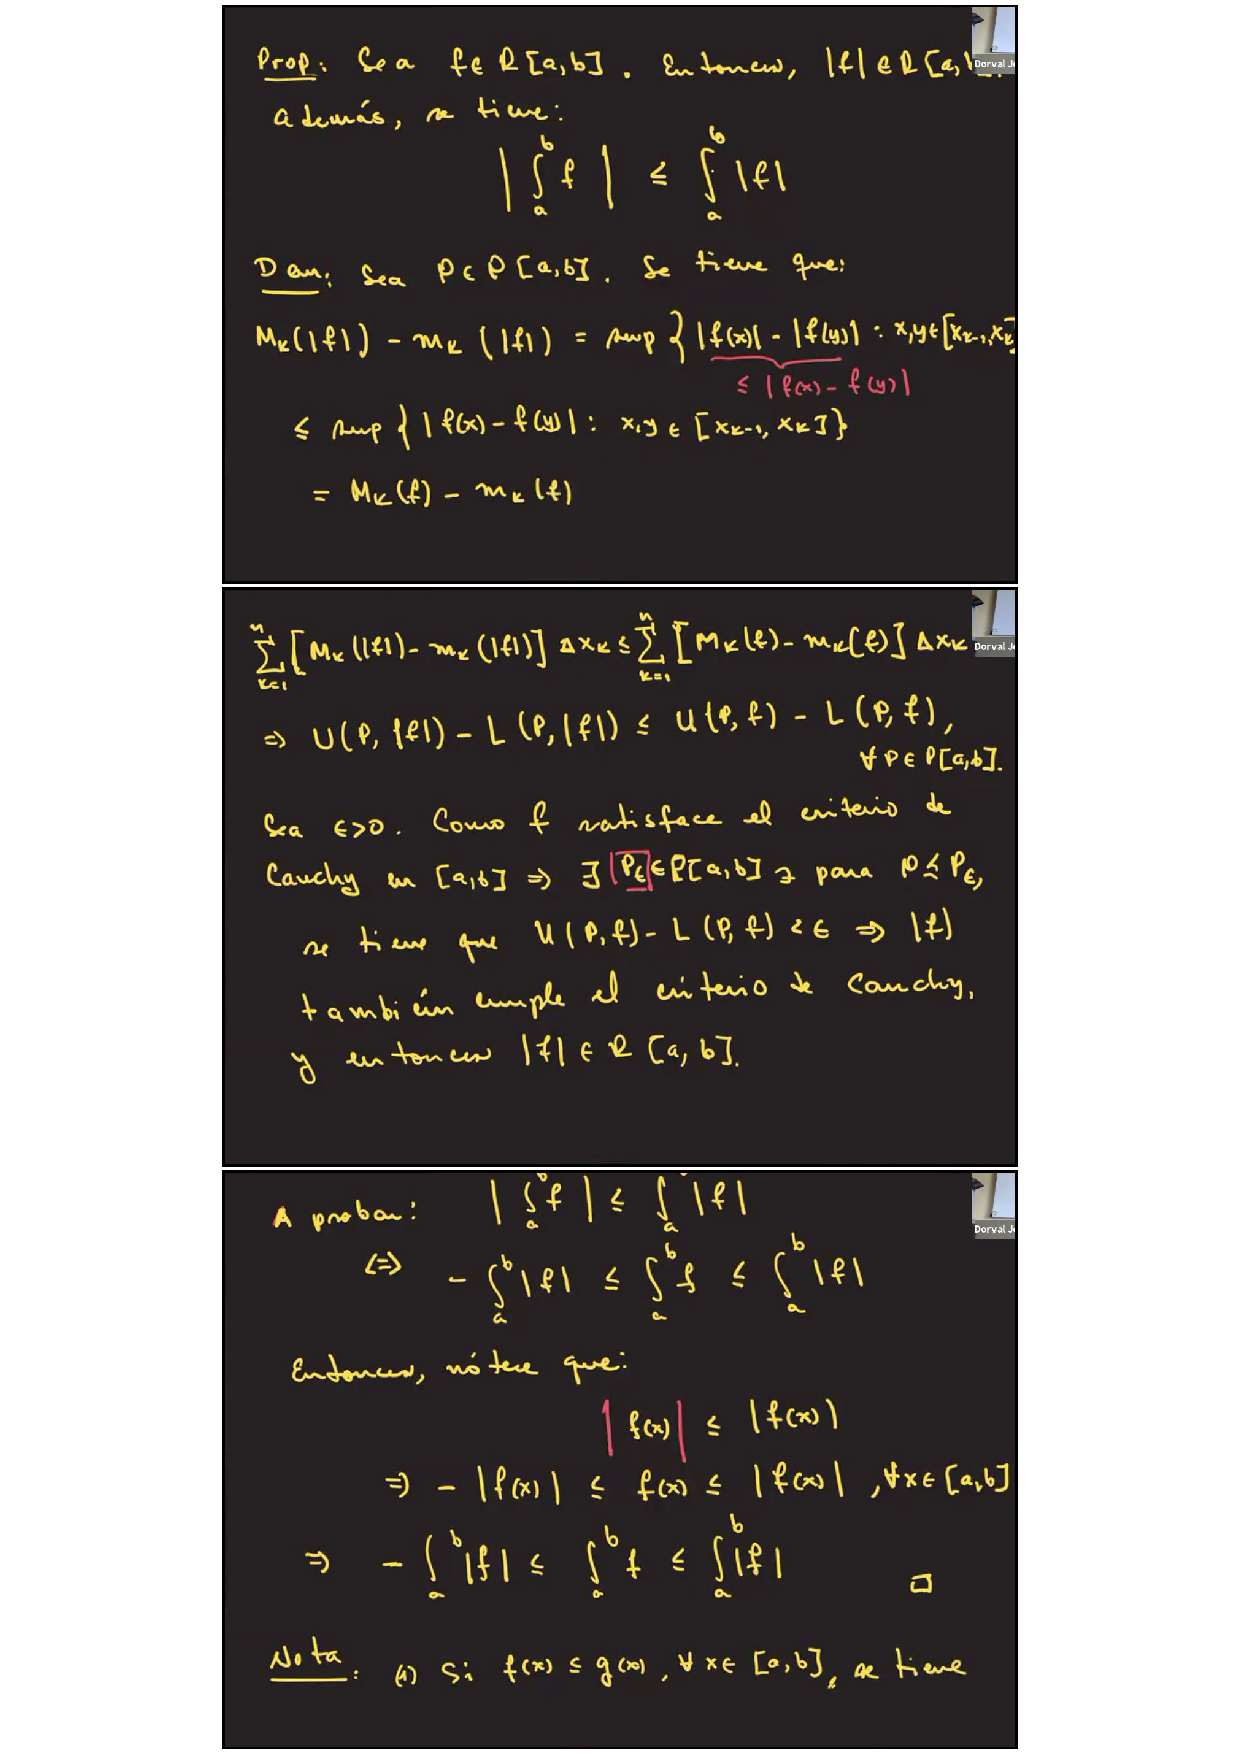
\includepdf[pages=-]{apendices/s5.pdf}